\section{Введение}

\textbf{Цель работы:}
измерение момента инерции ряда тел и сравнение результатов с расчетами
по теоретическим формулам; проверка аддитивности моментов инерции и
справедливости формулы Гюйгенса-Штейнера.

\textbf{В работе используются:}
трифилярный подвес, секундомер, счетчик числа колебаний, набор тел,
момент инерции которых надлежит измерить (диск, стержень, полый цилиндр
и другие).

Инерционность при вращении тела относительно оси определяется моментом
инерции тела относительно этой оси. Момент инерции твердого тела
относительно неподвижной оси вращения вычисляется по формуле
\begin{equation}
    I = \int r^2dm.
\end{equation}

Здесь $r$ — расстояние элемента массы тела dm от оси вращения.
Интегрирование проводится по всей массе тела $m$.
\begin{figure}[H]
    \centering
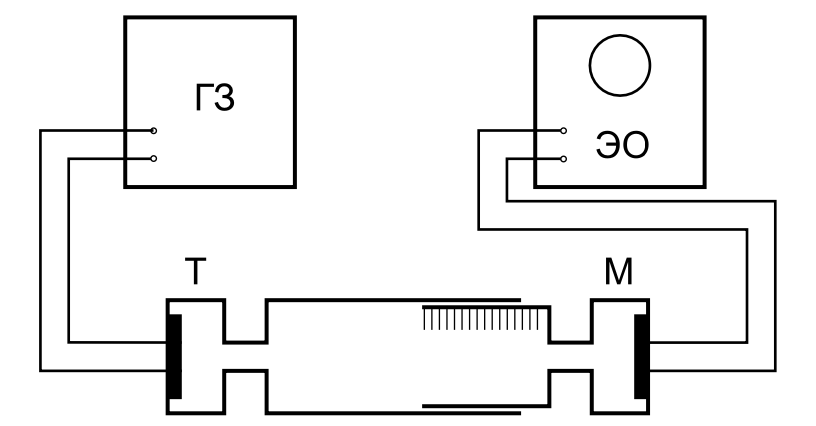
\includegraphics[width=0.5\linewidth,center]{p1.png}
    \caption{Трифилярный подвес}
    \label{fig:my_label}
\end{figure}

Для однородных тел известной плотности при заданных размерах и
достаточно простой форме момент инерции можно вычислить. Для
неоднородных тел и тел сложной формы момент инерции можно определить
экспериментально. Удобно использовать устройство, показанное на рис. 1
и называемое трифилярным подвесом. Оно состоит из укрепленной на
некоторой высоте неподвижной платформы $P$ и подвешенной к ней на трех
симметрично расположенных нитях $AA'$, $BB'$ и $CC'$ вращающейся
платформы $P'$.

Платформа $P$ укреплена на кронштейне и снабжена рычагом (на рисунке не
показан), при помощи которого в системе можно создать крутильные
колебания путем небольшого поворота верхней платформы. Лучше
поворачивать верхнюю платформу, укрепленную на неподвижной оси, чем
подвешенную на нитях нижнюю, так как нижнюю платформу трудно закрутить
не вызвав ее раскачиваний, подобных движению маятника, учет которых
сильно усложнил бы расчеты. После поворота, вызывающего крутильные
колебания, верхняя платформа остается неподвижной в течение всего
процесса колебаний. После того, как нижняя платформа $P'$ оказывается
повернутой на угол $\varphi$ относительно верхней платформы $Р$,
возникает момент сил, стремящийся вернуть нижнюю платформу в положение
равновесия, при котором относительный поворот платформ отсутствует. Но в
положении равновесия платформа не останавливается, так как имеет угловую
скорость (кинетическую энергию вращения). В результате платформа
совершает крутильные колебания.

Если пренебречь потерями энергии на трение (о воздух и в креплениях нитей), то уравнение сохранения энергии при колебаниях можно записать следующим образом:

\begin{equation}
    \frac{I\dot{\varphi}^2}{2} + mg \left(z_0 - z\right) = E.
\end{equation}

Здесь $I$ — момент инерции платформы вместе с исследуемым телом, $m$ —
масса платформы с телом, $\varphi$ — угол поворота платформы от
положения равновесия системы, точкой обозначена производная по времени
(угловая скорость), $z$ - координата по вертикали центра нижней
платформы $О'$ при равновесии $\left(\varphi = 0\right)$, $z$ —
координата той же точки при некотором угле поворота $\varphi$. Первый
член в левой части уравнения - кинетическая энергия вращения, второй
член - потенциальная энергия в поле тяжести, $E$ — полная энергия
системы (платформы с телом).

Отметим, что, как показывает соотношение (2), возвращающая сила
возникает благодаря силе тяжести.

Воспользуемся системой координат $x, y, z$, связанной с верхней
платформой, как показано на рис. 1. Координаты верхнего конца одной из
нитей подвеса точки $C$ в этой системе - $\left(r, 0,0 \right)$. Нижний
конец данной нити $C''$, находящийся на нижней платформе, при равновесии
имеет координаты $(R, 0, z_0)$, а при повороте платформы на угол
$\varphi$ эта точка переходит в $C''$ с координатами
$(R\cos{\varphi}, R\sin{\varphi}, z)$. Расстояние между точками $C$ и
$C''$ равно длине нити $L$. Поэтому

\begin{equation}
    \left(R\cos\varphi - r\right)^2 + R\sin^2\varphi + z^2 = R^2.
\end{equation}

Учитывая, что при малых углах
$\cos\varphi \approx 1 - \frac{\varphi^2}{2}$, получаем

\begin{equation}
    z^2 = L^2 - R^2 - r^2 + 2Rr\cos \varphi \approx = z_0^2 - Rr\varphi^2.
\end{equation}

Извлекая из (4) квадратный корень и учитывая малость угла $\varphi$, имеем

\begin{equation}
    z \approx z_0 -\frac{Rr\varphi^2}{2z_0}.
\end{equation}

Подставляя это значение $z$ в уравнение (2), получаем
\begin{equation}
    \frac 12I\dot{\varphi}^2+mg\frac{Rr}{2z_0}\varphi^2 = E.
\end{equation}
Дифференцируя по времени и сокращая на $\dot{\varphi}$, находим уравнение крутильных колебаний системы:

\begin{equation}
    I\ddot{\varphi} + mg \frac{Rr}{z_0}\varphi = 0.
\end{equation}

Период крутильных колебаний нашей системы равен:
\begin{equation}
    T = 2\pi \sqrt{\frac{Iz_0}{mgRr}}.
\end{equation}

Из формулы (8) находим момент инерции
\begin{equation}
    I = kmT^2.
\end{equation}

Здесь $k =\frac{gRr}{4\pi^2z_0}$ -- величина, постоянная для данной
установки.

Таким образом, полученные формулы позволяют определить момент инерции платформы с телом и отдельно платформы по соответствующим периодам крутильных колебаний. Затем вычисляем момент инерции тела, пользуясь аддитивностью, в справедливости которой можно убедиться, проведя измерения сначала для каждого из двух тел отдельно, а затем для обоих тел вместе.

При выводе формул предполагалось, что малы необратимые потери энергии, связанные с трением, то есть мало затухание колебаний. О затухании колебаний можно судить, сравнивая время $\tau$ уменьшения амплитуды колебаний в 2-3 раза с периодом колебаний $T$. Необратимыми потерями энергии можно пренебречь, если выполняется условие
\begin{equation}
    \tau \gg T
\end{equation}

В данной работе рекомендуется период колебаний определять с относительной погрешностью 0,5\%. Число колебаний, по которым надо вычислять период, определяется этой погрешностью и погрешностью измерения времени.

Для счета числа колебаний используется счетчик, состоящий из осветителя (2), фотоэлемента (3) и пересчетного устройства (1) (см. рис. 1). Легкий лепесток, укрепленный на платформе, при колебаниях пересекает световой луч дважды за период. Соответствующие сигналы от фотоэлемента поступают на пересчетное устройство.
